%===================================== CHAP 3 =================================

%\chapter{Method}
\chapter{Conceptual design}
%\chapter{Approach and methodology}

\section{Overall Approach}

%%forklare hva jeg prøver å gjøre på en generell måte. introdusere pipelinen
Wikipedia is a web page presenting articles for the user. This leads to high focus on the usability related to users searching and reading articles. Because of this one can say that their articles are stored as an atomic entity in their database. An articles has no internal structure, except for the markup used to present it. That means that a process is needed to identify and extract examples from Wikipedia articles. This 
project%%Hva burde jeg kalle dette?
looks into the pipeline technique for this process. As explained in section \ref{pipeline}, a pipeline consist of multiple independent processes loosely coupled.\\


%\section{Prerequisite knowledge}

\section{Pipeline}

%%Write something about the approach being for data mining. Where to different methods where explored. Focus on how it was done.
\subsection{Creating the pipeline} \label{custom-pipeline}

%%del opp deler av pipelinenen i subsectioen under denne sectionenen, del opp i SQL og elastic search. Ta med prosessen som fører til det

\begin{figure}[h]
\caption{A conceptual overview of the pipeline used to extract and index examples}
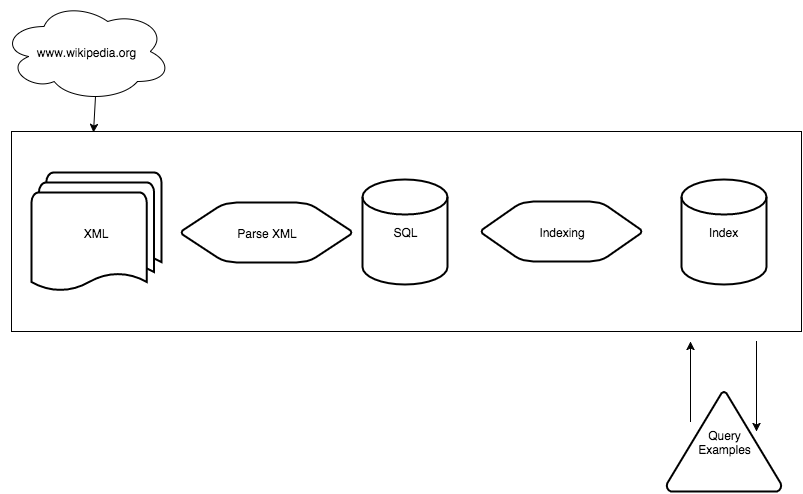
\includegraphics[width=\textwidth]{PipelineConcept}
\end{figure}



As described in section \ref{smila}, SMILA did not end up being a helpful tool for this project. Therefor other methods were considered, which mainly consisted of building the pipeline from scratch. Tailoring the different sub-processes for this project and organizing them in a pipeline, was decided to be the best course of action. The first issue to be settled regarded the format of the source data. SMILA was supposed to crawl www.wikipedia.org, but using a web-crawler is a very general method. Since this project were going to use wikipedia, it could be more specific. An XML-dump from a snapshot of wikipedias database was decided to be the best solution. This dump contains all the articles of wikipedia in their newest version.

All the sub-processes in the pipeline are loosely coupled. This means that they are fully independent given the correct input. This also allows the pipeline to easily swap out sub-processes without affecting the rest of the system. The SMILA pipeline also delivered a high degree of parallelity. This is a property the current version of the pipeline created from scratch does not have. This is because functionality was prioritized above efficiency during development. 

\subsection{Extracting data from XML-dump to SQL}
A parsing process was created in JavaScript running locally on a node.js server. This process iterates through every article and identifies sections with examples in them. It then parses that article into a JavaScript object with the relevant data. As it iterates over the articles, the process stores the data in a sql database with its new structure and relations. 

\subsection{Building an index of examples from SQL}
%write about elastic search



To allow an effortless fetching of data from the database a view was created. This view contains the fields that later in the pipeline will be used to build the index. Elasticsearch was chosen as tool for building the index. A simple java program fetches the view, containing the examples, from the database and builds an index. Elasticsearch serves a http API for querying of the index.



\section{Analysis of examples} %% må skrives om til hvordan vi faktisk drar nytte av det, når det blir implementert
%strucutre/characteristics of an example\\
%what is good and bad example

\subsection{An example}

An example is used as a tool to better understand a topic. It is usually used together with an explanatory text, where the example is a minor part of it. Examples are rarely presented standalone since they often required a certain degree of context. If this context is fused into the example, it often tends to make the example very complex and too troublesome to use efficiently. Because of this, an example can often be looked at as an appendix to a text regarding a subject. 


%%Finn et annet ord for persons?
Persons who want to learn about a certain topic, but already knows the basic context may prefer to skip the explanatory text and only look at the examples. This projects tries to exploit the fact that examples acts as an appendix to a subject and index them based on that. This attempts to give persons, trying to expand their knowledge within a topic, a more preferable way of doing so.

\subsection{Comparing examples} \label{comparing_examples}

To find common properties of examples is very difficult. Nearly impossible if you compare across different domains. When comparing two examples within the same domain and topic, there will still be different approaches and techniques of explaining, which still makes it hard to directly compare them. As a consequence of this, a highly qualitative and subjective analysis has been made for examples within the Game Theory domain. 

Different key properties have been identified and examined across different topics. Some properties are connected to the structure and presentation of the example, while others are based on the contents. From examining topics within Game Theory, a list of properties of an example were designed: Figures; Length; Domain; Source-code; Equations; Analogies; Subcategories under an example that explains the subject in different ways; Has a walkthrough or a step by step guide; Several iterations of the explanation, while gradually increase the complexity; References figures actively during the example.

%%Maybe the list above should be an appendix or table?


\subsection{Characteristics of a good example} \label{good_example}

When trying to identify the characteristics of a good example, there have been selected a few topics within the Game Theory domain. Then for a certain topic, two or three examples have been compared to each other.  

For the topic \textit{Pareto efficiency} the first example examined is\\ https://www.economics.utoronto.ca/osborne/2x3/tutorial/PEDEX.HTM. This example builds up its explanation step by step with several iterations. Each iteration is a bit more complex than the previous. This enables the example to cover the topic with a certain depth. The second example is https://www.tau.ac.il/~spiegel/teaching/inter-micro/Crueso.pdf. This example is very long and detailed. In addition to a large amount of text, it also uses equations to a substantial degree. Initially the first example feels better, it is definitely easier to grasp the concept of \textit{Pareto efficiency}. The second example focuses more on the mathematical part, and there will most likely exist some persons who prefer this. 

\subsection{Using the results}

As explained in section \ref{good_example}, the characteristics of a good example may change based on the person making use of it. For the index built in this project it is important to acknowledge this. By using the properties listed in section \ref{comparing_examples} and the characteristics of good examples, a smarter index can be created. Hopefully this will help the user search for examples for the relevant topic, and find related examples to improve the learning.

\cleardoublepage